%%%%%%%%%%%%%%%%%%%%%%%%%%%%%%%%%%%%%%%%%%%%%%%%%%%%%%%%%%%%%%%%%%%%%%%%%%%%%%
% Template LaTeX Template Version 1.0 (December 8 2014)
%
% This template has been downloaded from: http://www.LaTeXTemplates.com
%
% Original author: Brandon Fryslie With extensive modifications by: Vel
% (vel@latextemplates.com)
%
% License: CC BY-NC-SA 3.0 (http://creativecommons.org/licenses/by-nc-sa/3.0/)
%
% Authors: Sabbir Ahmed, Jeffrey Osazuwa, Howard To, Brian Weber
% 
%%%%%%%%%%%%%%%%%%%%%%%%%%%%%%%%%%%%%%%%%%%%%%%%%%%%%%%%%%%%%%%%%%%%%%%%%%%%%%

\documentclass[12pt]{extarticle}
%%%%%%%%%%%%%%%%%%%%%%%%%%%%%%%%%%%%%%%%%
% Structure
% Structural Definitions File
% Version 1.0 (December 8 2014)
%
% Created by:
% Vel (vel@latextemplates.com)
% 
% This file has been downloaded from:
% http://www.LaTeXTemplates.com
%
% License:
% CC BY-NC-SA 3.0 (http://creativecommons.org/licenses/by-nc-sa/3.0/)
%
%%%%%%%%%%%%%%%%%%%%%%%%%%%%%%%%%%%%%%%%%

\usepackage{geometry} % Required to modify the page layout

\usepackage{amsmath}
\usepackage{amssymb}

\usepackage[utf8]{inputenc} % Required for including letters with accents
\usepackage[T1]{fontenc} % Use 8-bit encoding that has 256 glyphs

\usepackage{avant} % Use the Avantgarde font for headings
\usepackage{setspace}

\setlength{\parindent}{0mm} % Don't indent paragraphs
\setlength{\parskip}{2.5mm} % Whitespace between paragraphs

\setlength{\textwidth}{16cm} % Width of the text on the page
\setlength{\textheight}{23cm} % Height of the text on the page
\setlength{\oddsidemargin}{0cm} % Width of the margin - negative to move text left, positive to move it right
\setlength{\topmargin}{-1.25cm} % Reduce the top margin

\renewcommand\familydefault{\sfdefault}  % default font for entire document
 % specifies the document layout and style
\usepackage{tabularx}
\usepackage{outlines}
% names
\newcommand{\team}{Galois Field Arithmetic Unit}
\newcommand{\Sabbir}{Sabbir Ahmed}
\newcommand{\Jeffrey}{Jeffrey Osazuwa}
\newcommand{\Howard}{Howard To}
\newcommand{\Brian}{Brian Weber}

% document info command
\newcommand{\documentinfo}[5]{
    \begin{centering}
        \parbox{6.8in}{
        \begin{spacing}{1}
            \begin{flushleft}
                \begin{tabular}{l l} #1 \\ #2 \\ #3 \\ #4 \\ #5 \\
                \end{tabular}\\
                \rule{\textwidth}{1pt}
            \end{flushleft}
        \end{spacing} }
    \end{centering} }

\graphicspath{ {diagrams/} }
\renewcommand{\baselinestretch}{1.5}
\setenumerate[1]{label=\textbf{\theparagraph.\arabic*.}, leftmargin=6em}
% \setenumerate[2]{label=\textbf{\thesubsubsection.\arabic*.}, leftmargin=6em}
% \renewcommand{\theenumi}{  %
%     \ifnum\value{paragraph}=0
%         \setenumerate[1]{label=\textbf{\thesubsubsection.\arabic*.},
%         leftmargin=6em}
%     \fi
% }

% \setenumerate[2]{label*=\arabic*.}

\begin{document}

    \documentinfo {\textbf{MEMO NUMBER:} GFAU SOW} {\textbf{DATE:} {\today}}
    {\textbf{TO: } EFC LaBerge} {\textbf{FROM: }\Sabbir, \Jeffrey, \Howard,
    \Brian} {\textbf{SUBJECT: } Galois Field Arithmetic Unit Statement of Work}
    \vspace{-0.3in}

    \section{Introduction} A Galois Field is a field with a finite number of
    elements. The nomenclature $GF(q)$ is used to indicate a Galois Field with
    $q$ elements. In $GF(q)$, the parameter $q$ must be a power of a prime. For
    each prime power there exists exactly one finite field. The binary field
    $GF(2)$ is the most frequently used Galois field \cite{wolfdef}.

    The \team~will handle irreducible polynomials in $GF(2^n)$, where $2 \leq
    n \leq 16$. The arithmetic logic unit (ALU) will generate all the terms in
    the field of the polynomial, and allow the user to view and apply the
    following Galois operations: addition, subtraction, multiplication,
    division and logarithm.

        \subsection{Purpose and Scope} This Statement of Work outlines and
        elaborates the tasks necessary to implement the project. The document
        also details their corresponding milestones and deadlines and how the
        contribution will be divided within the team.

    \section{Roles and Division of Labor} This project requires equal team work
    on all tasks because of the steep learning curve on implementing
    coprocessors with programmable boards. None of the team members have
    comprehensive prior knowledge or training on field programmable gate array
    units, and are therefore required to learn the concepts concurrently.

    Although there is no clear division of labor within the team, each members
    have been implicitly designated unofficial roles. Table \ref{table:roles}
    provides an estimated division of labor among the members of \team.

    \begin{table}[h]
        \renewcommand{\arraystretch}{1.5}
        \renewcommand{\baselinestretch}{1}
        \caption{Estimated Division of Labor of \team~}
        \centering

        \begin{tabularx}{\textwidth}{ | c | X | }
        \hline
        \textbf{Member} & \textbf{Responsibilities} \\
        \hline

        \textbf{Sabbir} & \noindent\parbox[c]{\hsize}{\begin{itemize}
            \item Validate the system inputs and outputs through the operations
            in the unit
            \item Provide background information on the mathematical concepts
            and theoretical design
            \item Finalize written reports and deliverables
        \end{itemize}} \\
        \hline

        \textbf{Jeffrey} & \noindent\parbox[c]{\hsize}{\begin{itemize}
            \item Design modules using the hardware description language
            \item Support the designing processes by providing test benches
            and by synthesizing the individual modules
        \end{itemize}} \\
        \hline

        \textbf{Howard} & \noindent\parbox[c]{\hsize}{\begin{itemize}
            \item Act as the point of contact between the team and the project
            manager and other consultants
            \item Schedule team meetings and milestones
        \end{itemize}} \\
        \hline

        \textbf{Brian} & \noindent\parbox[c]{\hsize}{\begin{itemize}
            \item Maintain and validate the digital design of the system at
            various levels
            \item Oversee the designing of the system using the hardware
            description language
            \item Finalize written reports and deliverables
        \end{itemize}} \\
        \hline

        \end{tabularx}
        \label{table:roles}
    \end{table}

    Along with the assigned responsibilities, each members of the GFAU shall
    contribute to programming the individual modules in the system. Each
    members shall also contribute to authoring the documents supporting the
    project design and requirements.

    \section{Tasks}

        \subsection{Research} The initial set of tasks relate to research
        efforts to fully understand the requirements and develop an
        implementation of the GFAU.

            \subsubsection{Background} The team shall conduct research on the
            mathematics and theoretical concepts related to Galois fields. The
            GFAU generates terms in specified Galois fields and stores them for
            further operations. Therefore, a strong understanding on such
            topics is essential for successful and accurate computations.

            \subsubsection{Devices} The team shall conduct research on the
            implementation and synthesis of digital design on programmable
            boards and their corresponding best practices.
            
                \paragraph{Field Programmable Gate Array (FPGA)} \leavevmode
                \\~\\ The team shall conduct research to address the following
                inquiries regarding FPGA development boards and design.
                \begin{enumerate}
                    \item The team shall conduct trade studies on designs
                    commonly used for arithmetic operations which are performed
                    in the GFAU.
                    \item The team shall identify styles and best practices for
                    hardware synthesizable VHDL code.
                    \item The team shall identify hardware specifications
                    deemed important before purchase.
                    \item The team shall identify hardware specifications to
                    meet the requirements detailed in the System Requirements
                    Specifications.
                \end{enumerate}

                \paragraph{External Devices} \leavevmode \\~\\ The team shall
                conduct research to address the following inquiries regarding
                external devices interfacing the FPGA development board.

                \begin{enumerate}
                    \item The team shall identify the external devices suitable
                    for interfacing the GFAU.
                    \item The team shall conduct a study of protocols commonly
                    used to communicate with coprocessors to determine how to
                    communicate with the widest range of the most commonly used
                    microprocessors.
                    \item The team shall identify hardware specifications of
                    the external devices to meet the requirements detailed in
                    the System Requirements Specifications.
                \end{enumerate}

        \subsection{Design}

            \subsubsection{System Boundary} The team shall design a system
            boundary diagram detailing the functions, inputs and outputs of the
            system. The team shall also develop and maintain additional
            diagrams elaborating various hierarchical and functional views of
            the project, including the functional flow and data flow diagrams.

            \subsubsection{Schematics} The team shall develop 
            schematics and other documentation necessary for the development
            phase. For the final product, the team shall develop a high-level
            schematic consisting of all the modules in the system. The
            schematic shall be divided into segments to be elaborated on a
            lower level by individual members.
            
            \subsubsection{System Design Document} The team shall compile a
            System Design Document detailing the architectural, logical and
            physical design of every level of the system.

        \subsection{Software Implementation}

            \subsubsection{Design in VHSIC Hardware Description Language
            (VHDL)} The team shall implement independent and discrete VHDL
            modules for each of the operations in the GFAU. The source
            code shall be written and comprehensively documented using the best
            practices and standards imposed by the \textit{IEEE Standard VHDL
            Language Reference Manual} (2009).

            \subsubsection{Simulation and Synthesis in VHDL} The team shall
            test each module after completion to minimize syntax and
            implementation warnings and errors. Individual test benches shall
            be written to accompany their corresponding module for every module
            in the system. The team shall complete the modules using using
            syntax that is synthesizable for use in the chosen FPGA. Each
            module shall be independently synthesized to ensure they match the
            intended schematics and designs. The team should complete all
            simulations and software testing by the end of December.

            \subsubsection{External Devices} The system may require external
            devices, such as memory. The team shall abstract and simulate their
            behavior in VHDL before the physical integration to validate their
            functionality. The VHDL code written to describe the behavior of
            external devices does not necessarily have to be synthesizable.

            \paragraph{External Device Library} \leavevmode \\~\\ The team may
            provide a library for the external device to interface the GFAU
            system. The library may include methods, protocols and constants to
            establish communication with and send and receive signals to the
            GFAU prototype.

        \subsection{Purchases} Before purchase, the team shall conduct research
        on external memory chips suitable for storing the lookup tables created
        during the polynomial term generation. Research on the external memory
        interface includes simulation and testing of its truth tables using
        VHDL. The team shall concurrently conduct research to find a
        development board which satisfies the requirements outlined in the
        System Requirements Document.

        \subsection{Hardware}

            \subsubsection{Integration} The team shall integrate the system
            with an FPGA board bounded by the constraints detailed in the
            Systems Requirement Specifications. The board shall successfully
            communicate with a microcontroller for user interface and its
            external memories. The team shall complete the hardware integration
            phases by mid-spring after all final purchases.

            \subsubsection{Hardware Testing} The team shall continuously test
            the FPGA board and its external components before, during and
            after the integration with the VHDL system modules. The testing of
            the hardware in the system shall serve as the final milestone for
            the project during the end of the spring semester.

            \begin{enumerate}[label=\textbf{\thesubsubsection.\arabic*.},
            leftmargin=6em]
                \item The team shall conduct logical tests of the prototype
                using a Digital Logic Analyzer to verify the logical
                correctness and timing constraints of the GFAU.
                \item The team shall conduct testing of both input and output
                signals using an oscilloscope to verify all signals going in
                and out of the GFAU meet the requirements outlined in Section
                3.5 of the System Requirements Specification.
            \end{enumerate}

    \newpage
    \section{Deliverables} Table \ref{deliverables} details the expected
    deliverables throughout the project and shall be completed concurrently
    with the project development.

    \begin{table}[h]

        \renewcommand{\arraystretch}{1.8}
        \caption{Deliverables}
        \centering

        \begin{tabular}{ | p{10em} | p{16em} | l |}

            \hline \textbf{Deliverable} & \textbf{Description} &
            \textbf{Deadline} \\

            \hline \textbf{System Specification Requirements} & The team shall
            develop a detailed specification of the unit. The specification
            document shall include both hardware and software requirements and
            constraints. The System Specification Requirements also detailed
            all the inputs and outputs of the GFAU. & November 22nd, 2017 \\

            \hline \textbf{Weekly Team Status Reports} & The team shall deliver
            bimonthly status reports to Dr. LaBerge discussing the completed
            tasks and issues encountered during the period. They shall also
            include planned tasks for the next period. & Bimonthly \\

            \hline \textbf{Preliminary Design Review} & The team shall present
            a Preliminary Design Review of the project to Dr. LaBerge in the
            first week of December. & December 6th, 2017 \\

            \hline \textbf{Completed Design Review} & The team shall present a
            final review of the GFAU to Dr. LaBerge and others in May, 2018. &
            May, 2018 \\

            \hline \textbf{Demo} & The team shall present a fully functional
            demo of the GFAU to Dr. LaBerge and others in May, 2018. & May,
            2018 \\

            \hline

        \end{tabular}
    \label{deliverables}
    \end{table}

    \section{Timeline} Figure 1 below shows a timeline of the capstone project
    in a Gantt Chart.

    \begin{figure}[h]
        \begin{center}
            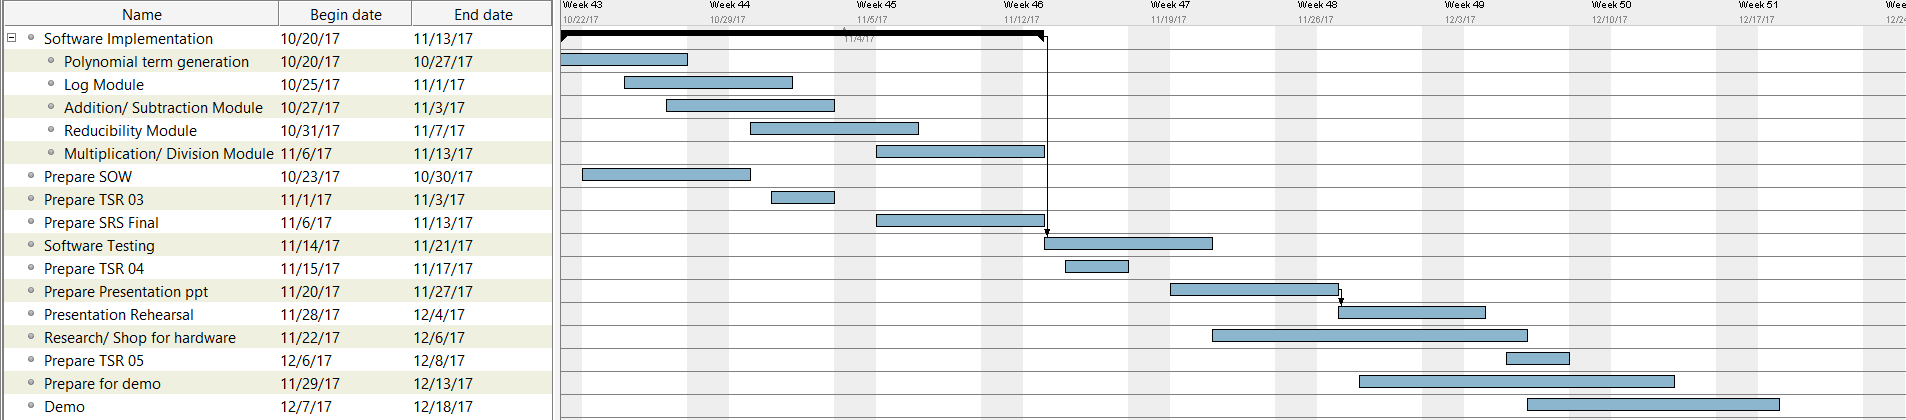
\includegraphics[width=1\textwidth]{gantt_chart.png}
            \caption{Capstone Schedule} \label{fig:gantt_chart}
        \end{center}
    \end{figure}

    \begin{thebibliography}{2}
        \bibitem{wolfdef}
        Wolfram Math World, "Finite Field." \textit{Wolfram Math World},
        2017. [Online document]. Availble:
              http://mathworld.wolfram.com/FiniteField.html. [Accessed:
              \today].

        \bibitem{ieeemanual}
        Design Automation Standards Committee of IEEE Computer Society,
        \textit{IEEE Standard VHDL Language Reference Manual}, IEEE Computer
        Society, 2009.
    \end{thebibliography}

\end{document}
